\section{The uniform rate and its sharp constant}\label{sec:rates}

The square-root correction has a uniform error of order $N^{-1/4}$. Its first signed term depends on parity, and the largest error has an explicit asymptotic constant. Retain $K=2\lfloor k/2\rfloor$, $\epsilon=k-K$ and $H_k$ from \eqref{eq:hyperdef}, and put
\begin{equation}\label{eq:rateW}
W_{N,k}=\frac{R_k}{e^{k^2/(4N)}H_k}.
\end{equation}

\begin{theorem}[An explicit uniform rate]\label{thm:rate}
For every fixed $C>0$,
\begin{equation}\label{eq:uniformrate}
\sup_{2\le k\le C\sqrt N}|W_{N,k}-1|=O_C(N^{-1/4}).
\end{equation}
More precisely, the explicit constants $A_i(C)$ in \eqref{eq:rateconstantsA} satisfy
\begin{equation}\label{eq:ratefinite}
|W_{N,k}-1|
\le A_1(C)N^{-1/4}+A_2(C)N^{-1/2}+A_3(C)N^{-1}
\end{equation}
whenever $N\ge16C^2$ and $2\le k\le C\sqrt N$. In addition, $A_1(C)\to0$ as $C\downarrow0$.
\end{theorem}

Appendix~\ref{sec:rateproof} proves the finite estimate, including fixed orders and the odd small-$\lambda$ regime. The constants are conservative. Their behavior as $C\downarrow0$ lets the following first correction remain uniform down to the smallest orders.

Define, for $c\ge0$,
\begin{equation}\label{eq:ratepsi}
\psi_\epsilon(c)=\frac{2\epsilon-1}{2}\sqrt c+\frac{2}{15}c^{5/2}.
\end{equation}

\begin{theorem}[Uniform first correction and sharp error constant]\label{thm:firstcorrection}
For every fixed $C>0$,
\begin{equation}\label{eq:uniformfirstcorrection}
\sup_{2\le k\le C\sqrt N}
\left|N^{1/4}(W_{N,k}-1)-\psi_{k\bmod2}(k/\sqrt N)\right|
\longrightarrow0.
\end{equation}
Consequently,
\begin{equation}\label{eq:sharprateconstant}
\lim_{N\to\infty}N^{1/4}
\sup_{2\le k\le C\sqrt N}|W_{N,k}-1|
=\frac{\sqrt C}{2}+\frac{2}{15}C^{5/2}.
\end{equation}
All suprema are over integers. Thus the order in \eqref{eq:uniformrate} is optimal for every fixed $C>0$.
\end{theorem}
\begin{proof}
Fix $0<d<C$. On $d\sqrt N\le k\le C\sqrt N$, the hypotheses of \eqref{eq:logsublinear} hold uniformly for sufficiently large $N$. Its remainder is $O_{C,d}(N^{-1/2})$. The series \eqref{eq:actionG} and the logarithm expansion give
\begin{align*}
NG(\sqrt{k/N})-\frac{k^2}{4N}
&=\frac{2k^{5/2}}{15N^{3/2}}+O_C(N^{-1/2}),\\
(\epsilon-1/2)\log(1+\sqrt{K/N})
&=\frac{2\epsilon-1}{2}\sqrt{k/N}+O_{C,d}(N^{-1/2}).
\end{align*}
The change from $K$ to $k$ in the second line costs at most a constant times $1/\sqrt{NK}$, which is smaller than the displayed remainder. Therefore
\[
\log W_{N,k}
=N^{-1/4}\psi_\epsilon(k/\sqrt N)+O_{C,d}(N^{-1/2}).
\]
The leading function is bounded on $[d,C]$. Exponentiation gives \eqref{eq:uniformfirstcorrection} uniformly on this restricted range.

For the remaining orders, \eqref{eq:ratefinite} with endpoint $d$ yields
\[
\limsup_{N\to\infty}N^{1/4}
\sup_{2\le k\le d\sqrt N}|W_{N,k}-1|\le A_1(d).
\]
Also $|\psi_\epsilon(c)|\le\sqrt d/2+2d^{5/2}/15$ for $0\le c\le d$. Split the full supremum at $d\sqrt N$, then let $d\downarrow0$. Since $A_1(d)\to0$, this proves \eqref{eq:uniformfirstcorrection}, including fixed orders and changing parity.

Finally,
\[
|\psi_0(c)|\le\psi_1(c)\le\psi_1(C)
=\frac{\sqrt C}{2}+\frac{2}{15}C^{5/2}
\qquad(0\le c\le C).
\]
The odd function is continuous and strictly increasing. Taking the largest odd integer $k_N\le C\sqrt N$ gives $k_N/\sqrt N\to C$. Equation~\eqref{eq:uniformfirstcorrection} supplies the matching lower limit, while its uniform bound supplies the upper limit. This proves \eqref{eq:sharprateconstant}.
\end{proof}

For example, at $k/\sqrt N\to1$, the signed limits are $-11/30$ along even orders and $19/30$ along odd orders. The sign change comes from the parity factor in \eqref{eq:logsublinear}. The positive $2c^{5/2}/15$ term is the first omitted term of the correction exponent. The sharp asymptotic constant in \eqref{eq:sharprateconstant} does not assert optimality of the finite constants $A_i(C)$.

\begin{figure}[htbp]
\centering
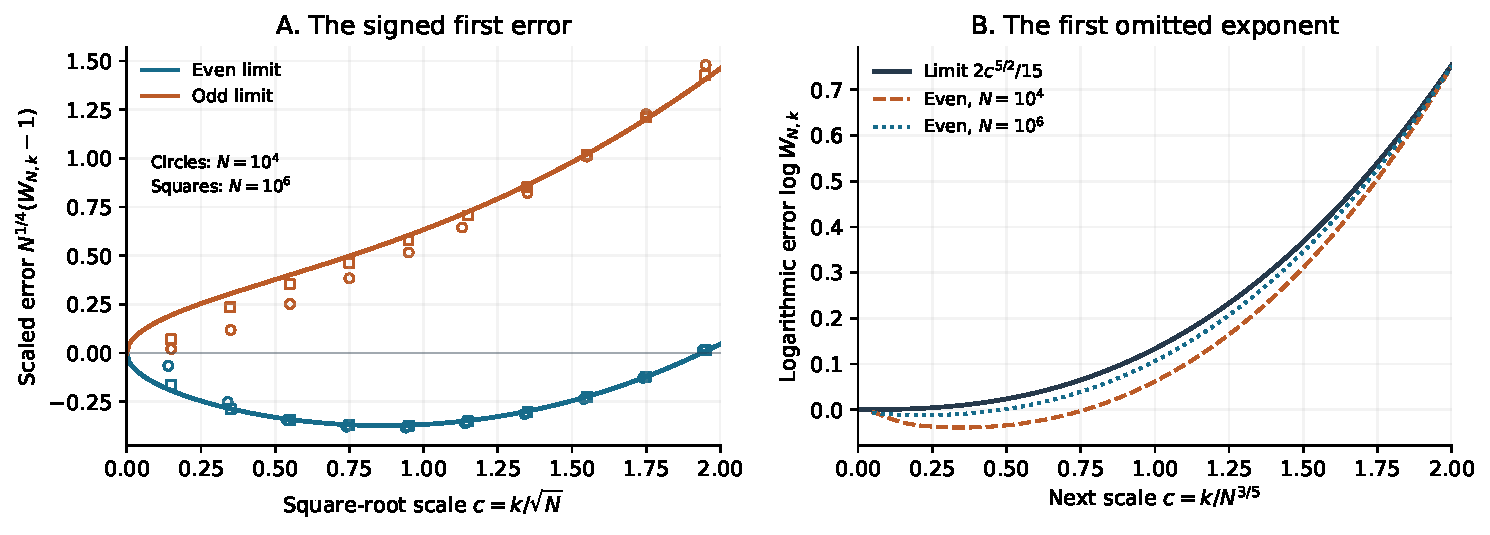
\includegraphics[width=\textwidth]{../figures/rate-and-hierarchy.pdf}
\caption{Two views of the next error. Left: the signed functions $\psi_0(c)$ and $\psi_1(c)$, compared with the positive recurrence at $N=10^4$ and $10^6$. Right: $\log W_{N,k}$ at $k\sim cN^{3/5}$ approaches $2c^{5/2}/15$. These finite evaluations corroborate the general theorems and are not used in their proofs.}
\label{fig:ratehierarchy}
\end{figure}
